\section{Margules activity model}

\subsection{Enthalpy and entropy of mixing}

The total change in Gibbs free energy due to mixing $\Delta G_{mix}$ using the
Margules activity model is
\begin{equation}\label{eq:margules}
    \Delta G_{mix} = RT[x_1 \ln x_1 + x_2 \ln x_2] + RTx_1x_2[A_{21}x_1 +
    A_{12}x_2].
\end{equation}

The entropy of mixing can be derived as
\stepcounter{equation}
\begin{align*}\label{eq:entrp1}
    -\Delta S_{mix} &= \qty(\pdv{\Delta G_{mix}}{T})_P = R[x_1\ln x_1 + x_2\ln
    x_2] + Rx_1x_2[A_{21}x_1 + A_{12}x_2] \\&\qquad\qquad + RTx_1x_2 \qty[ 
    \qty(\pdv{A_{21}}{T})_Px_1 + \qty(\pdv{A_{12}}{T})_Px_2] \\
    &= \dfrac{\Delta G_{mix}}{T} + RTx_1x_2 \qty[ 
    \qty(\pdv{A_{21}}{T})_Px_1 + \qty(\pdv{A_{12}}{T})_Px_2]. 
    \tag{\theequation}
\end{align*}

At the infinite dilution limit,
\begin{equation}\label{eq:ln-inf}
    \mu^\infty = \mu^\circ + RT\ln x + RT\ln \gamma^\infty \implies
    \ln \gamma^\infty = \dfrac{\mu^\infty - \mu^\circ}{RT} - \ln x.
\end{equation}

From Equations~\ref{eq:inf-dil} and \ref{eq:ln-inf}, we have
\begin{equation}\label{eq:enth1}
    \qty(\pdv{\ln \gamma_1^\infty}{T})_P = \frac1R\qty[\pdv{\mu_1^\infty/T}{T} -
    \pdv{\mu_1^\circ/T}{T}]_P = -\dfrac{\bar H_1^\infty - \bar H_1^\circ}
    {RT^2},
\end{equation}
where we have used the Gibbs--Helmholtz equation
\[
    \qty(\pdv{\mu/T}{T})_P = -\dfrac{\bar H}{T^2}.
\]
Similarly,
\begin{equation}\label{eq:enth2}
    \qty(\pdv{\ln \gamma_2^\infty}{T})_P = -\dfrac{\bar H_2^\infty - \bar H_2^\circ}
    {RT^2}.
\end{equation}

From Equations~\ref{eq:enth1} and \ref{eq:enth2}, we have that the partial
derivatives in Equation~\ref{eq:entrp1} can be expressed using partial molar
enthalpies at the standard state of a pure liquid $\bar H^\circ$ and the
partial molar enthalpy at the infinite dilution limit $\bar H^\infty$. Let the
difference between them be $\Delta \bar H^\infty$
\[
    \Delta \bar H^\infty \equiv \bar H^\infty - \bar H^\circ.
\]
We note that $\Delta \bar H^\infty$ depends on the liquid pair $\{1,2\}$ to
be mixed.

Finally, using Equation~\ref{eq:inf-dil}, we can recover another from of 
Equation~\ref{eq:entrp1} as
\begin{equation}\label{eq:entrp2}
    -\Delta S_{mix} = \dfrac{\Delta G_{mix}}{T} - \dfrac{x_1x_2}{T} \qty[
    \Delta \bar H_2^\infty x_1 - \Delta \bar H_1^\infty x_2].
\end{equation}

The enthalpy of mixing can then be expressed as
\begin{equation}\label{eq:enthalp}
    \Delta H_{mix} = \Delta G_{mix} + T\Delta S_{mix} = x_1x_2 \qty[
    \Delta \bar H_2^\infty x_1 - \Delta \bar H_1^\infty x_2].
\end{equation}
Having ``cross'' terms (the difference in subscripts) makes explicit the fact
that the different particles are interacting and that the strength of the
interactions depends on the mole fractions $x_i$ of the components.

An interpretation of the empirically fit coefficients then would be that they
represent \textit{collective} interactions between molecules that affect both
the enthalpy and entropy of the system due to mixing. These interactions can
include attraction and repulsion (enthalpic) and attractions related to size
(entropic).

\subsection{Liquid--liquid phase splitting}

By the second law of thermodynamics, a stable equilibrium state of the mixing
process would be a state that gives a local minimum for $\Delta G_{mix}$. Since
$\Delta G_{mix}$ is a function of $T, P, x_1$, given some parameters $A_{21}$
and $A_{21}$, we can choose to define $\Delta G_{mix}$ at some given $T,P$.
\[
    \Delta G_{mix} = \Delta G_{mix}(x_1; A_{21}, A_{12}).
\]
A necessary condition for a local extremum at $x_1 = \bar x_1$ would be
\[
    \pdv{\Delta G_{mix}}{x_1}\Bigg\rvert_{\bar x_1} = 0.
\]

Following from Equation~\ref{eq:margules}, the partial derivative is
\stepcounter{equation}
\begin{align*}\label{eq:gderv}
    \dfrac{1}{RT} \pdv{\Delta G_{mix}}{x_1} &= \ln \dfrac{x_1}{x_2} + 
    [A_{21}x_1 + A_{12}x_2](x_2 - x_1) + x_1x_2(A_{21} - A_{12}) \\
    &= \ln\dfrac{x_1}{1-x_1} + [A_{21}x_1 + A_{12}(1-x_1)](1-2x_1) +
    (x_1 - x_1^2)[A_{21} - A_{12}] \\
    &= \ln\dfrac{x_1}{1-x_1} + A_{12}(1-2x_1) 
    + [A_{21} - A_{12}](2x_1 - 3x_1^2). \tag{\theequation}
\end{align*}

By inspection of the equation above, the derivative of the free energy of
mixing is dependent on the difference $A_{21} - A_{12}$ (third term). 

\paragraph{Symmetric case}
The equilibrium condition for the case where $A_{21}=A_{12} \equiv A$ would be
\begin{equation}\label{eq:symm}
    \ln \dfrac{\bar x_1}{1-\bar x_1} + A(1 - 2\bar x_1) = 0 \implies
    \ln \dfrac{\bar x_1}{1-\bar x_1} = A(2\bar x_1 - 1).
\end{equation}

A solution would be $\bar x_1 = \bar x_2 = \frac12$ for any value of $A$. 
Suppose, $\bar x_1 \neq \bar x_2$, Equation~\ref{eq:symm} can be rearranged as
\begin{equation}\label{eq:symm2}
    f(\bar x_1) \equiv \dfrac{\ln \frac{\bar x_1}{1-\bar x_1}}{2\bar x_1 - 1} 
    = A = 
    \dfrac{\ln \frac{\bar x_1}{\bar x_2}}{\bar x_1 - \bar x_2},
\end{equation}
depending on the fit parameter $A$.

The function $f(\bar x_1)$ can be plotted against values of $\bar x_1$ as in 
Figure~\ref{fig:fx1}. It can be observed that at the function is not defined
at $\bar x_1 = \frac12$ as expected, yet the two-sided limit exists. The graph 
is also symmetric about $\bar x_1 = \frac12$ in the range $(0,1)$. This is 
expected since switching $x_1$ and $x_2$ in the last expression in 
Equation~\ref{eq:symm2} yields the same value.

\begin{figure}[ht]
    \centering
    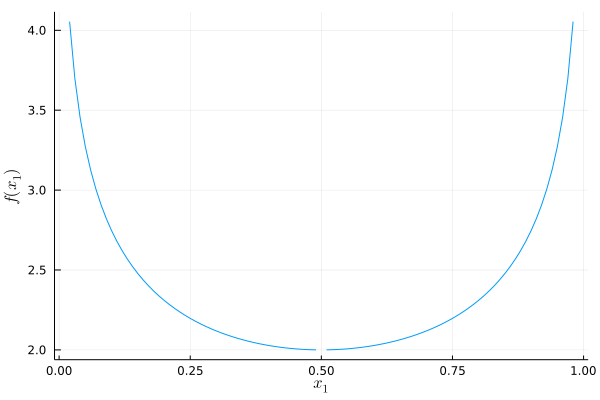
\includegraphics[scale=0.5]{./figs/fx1.png}
    \caption{A plot of $f(x_1)$ against $x_1$.}
    \label{fig:fx1}
\end{figure}

Within the physical range $x_1 \in (0,1)$, the infimum $\inf{f(\bar x_1)}$ is 
$2$.  The horizontal line $A = A_{21} = A_{12}$ crosses the graph of $f(x_1)$ 
twice when $A > 2$. This suggests that, including the trivial extremum at 
$\bar x_1=\frac12$, $\Delta G_{mix}$ has three extrema.
This suggests that for values $A>2$, there is a possibility of liquid--liquid 
phase splitting. For the following discussion we assume $A > 2$.

We prove that there is liquid--liquid phase splitting for $A > 2$.

Liquid--liquid phase splitting can happen when there are two local minima for
$\Delta G_{mix}(x_1)$ separated by a local maximum. The condition for a 
local minimum at an extremum $x_1 = \bar x_1$ is
\begin{equation}\label{eq:concav}
    \frac1{RT}
    \pdv[2]{\Delta G_{mix}(x_1)}{x_1}\Bigg\rvert_{\bar x_1} = 
    \dfrac{1}{\bar x_1(1-\bar x_1)} - 2A > 0 
    \implies 1 > 2A\bar x_1\bar x_2 = 2\bar x_1\bar x_2f(\bar x_1)
\end{equation}

Substituting $\bar x_1 = \frac12$ leads to a false inequality $A < 2$ 
for any $A>2$.
This suggests that there is a local maximum at $x_1 = \frac12$. A plot of the
rightmost expression in Equation~\ref{eq:concav} is given in 
Figure~\ref{fig:product}. It can be seen that the criterion in Equation
\ref{eq:concav} is satisfied for all extrema not equal to $\frac12$ when $A>2$.

Since there is a local maximum of $\Delta G_{mix}$ at $x_1=\frac12$ and there
are local minima $x_1'$ and $x_1''$ \textit{evenly} spaced from $x_1=\frac12$,
a \textit{symmetric} phase splitting can occur for $A>2$.

\begin{figure}[ht]
    \centering
    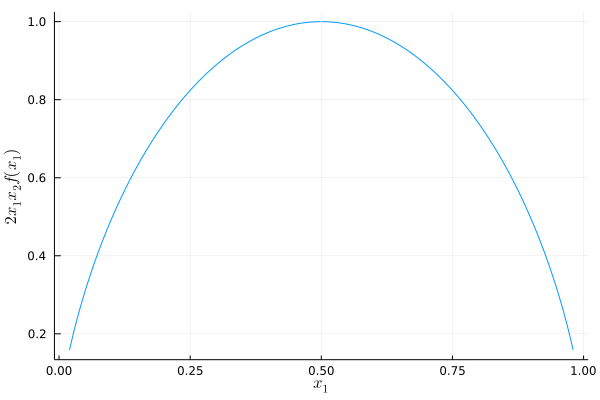
\includegraphics[scale=0.5]{./figs/fx2.png}
    \caption{A plot of $2f(x_1)x_1(1-x_1)$ against $x_1$.}
    \label{fig:product}
\end{figure}

\paragraph{Asymmetric case}
We consider roughly the same treatment for the case $A_{21} \neq A_{12}$.
We require that the derivative in Equation~\ref{eq:gderv} be zero at an
extremum $x_1 = \bar x_1$
\stepcounter{equation}
\begin{alignat*}{2}\label{eq:asymm}
    \MoveEqLeft \ln\dfrac{\bar x_1}{1-\bar x_1} + A_{12}(1-2\bar x_1) 
    + [A_{21} - A_{12}](2\bar x_1 - 3\bar x_1^2) = 0 \\
    &\implies
    \ln\dfrac{\bar x_1}{1-\bar x_1} = A_{12}(2\bar x_1 - 1) + 
    [A_{21} - A_{12}](3\bar x_1^2-2\bar x_1^2). \tag{\theequation}
\end{alignat*}

